\documentclass{article}
\usepackage[utf8]{inputenc}
\usepackage{subcaption}
\usepackage{graphicx}
\usepackage[margin=2.5cm]{geometry}
\usepackage{array}
\usepackage{wrapfig}
\usepackage{multirow}
\usepackage{tabularx}
\usepackage{amsmath}
\usepackage{wrapfig}
\usepackage{mathtools}
\usepackage[table]{xcolor}
\usepackage{xcolor,colortbl}
\usepackage{multirow}
\usepackage{polski}
\title{Ćwiczenie: 8}

\author{AUTOR}
\date{}
\begin{document}

\maketitle
%------------------------------------------------------------------
% WSTEP TEORETYCZNY
\section{Wstęp Teoretyczny}
\par Pomiar współczynnika lepkości $\eta$ cieczy metodą Stokesaza za pomocą 
szerokiego cylindrycznego 
naczynia szklanego. \\
\begin{center}
    $
    \eta=\frac{d^{2}\cdot g\cdot t\cdot (\rho_{k}-\rho_{c})}{18h}
    $
    \begin{flushleft}
        Gdzie:\\
        $d$ - średnica kulki\\
        $g$ - przyspieszenie ziemskie $(9.81\frac{m}{s^{2}})$\\
        $\rho_{k}$ - gęstość kulki\\
        $\rho_{c}$ - gęstość cieszy (gliceryny)\\
        $h$ - długość trasy tonącej w glicerynie kulki
    \end{flushleft}
\end{center}
\par Lepkość zostanie wyznaczona na podstawie danych otrzymanych przez obserwacje kulki 
tonącej w glicerynie. Dzięki analizie ruchu kulki, znając jej parametry takie 
jak masa i średnica, które przekładają się na gęstość. Można zanalizować siły oporu,
które stawia ciecz co przekłada się na współczynnik lepkości $\eta$.
\vspace{5ex}
\begin{figure}[h!]
    W naszym eksperymencie wykorzystamy następujące przyrządy:
    \begin{itemize}
        \item Naczynie cylindryczne z badaną cieczą (w tym wypadku z gliceryną)
        \item Areometr do zbadania gęstości cieczy
        \item Trzy różne kolorowe kulki (Biała, Czarna i Niebieska)
        \item Waga
        \item Suwmiarka do pomiaru średnicy kulek
        \item Stoper
        \item Linijka z podziałką milimetrową
    \end{itemize}


\end{figure}

% WSTEP TEORETYCZNY
%------------------------------------------------------------------
\newpage
%------------------------------------------------------------------
% OTRZYMANE POMIARY I ICH OPRACOWANIE
\section{Otrzymane pomiary i ich opracowanie}
%tabelki sa zjebane
\begin{figure}[h!]

    \begin{subfigure}{0.5\textwidth}
        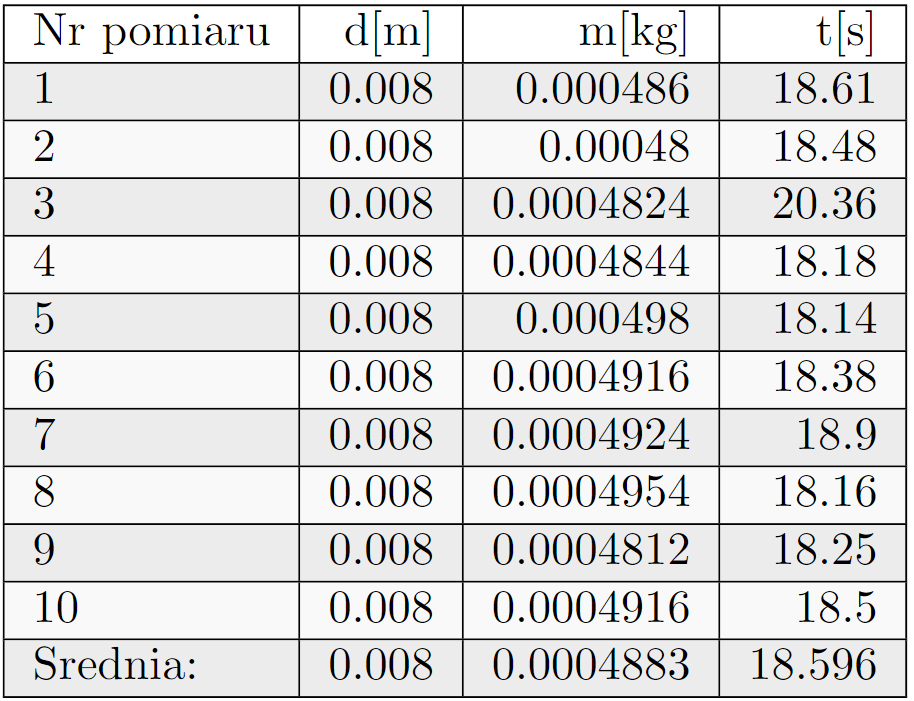
\includegraphics[width=0.9\linewidth, height=5cm]{t_biala_pom.png} 
        \caption{Pomiary kulki Białej}
        \label{fig:subim1}
    \end{subfigure}
    \begin{subfigure}{0.5\textwidth}
        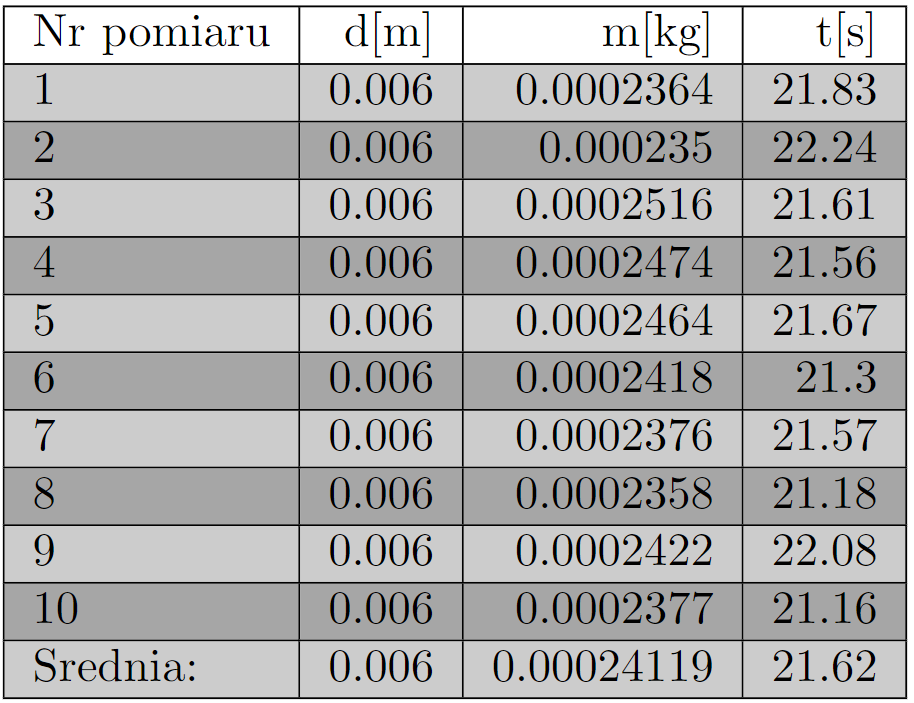
\includegraphics[width=0.9\linewidth, height=5cm]{t_czarna_pom.png}
        \caption{Pomiary kulki Czarnej}
        \label{fig:subim2}
    \end{subfigure}
    \begin{center}
        
        \begin{subfigure}{0.5\textwidth}
            \centering
        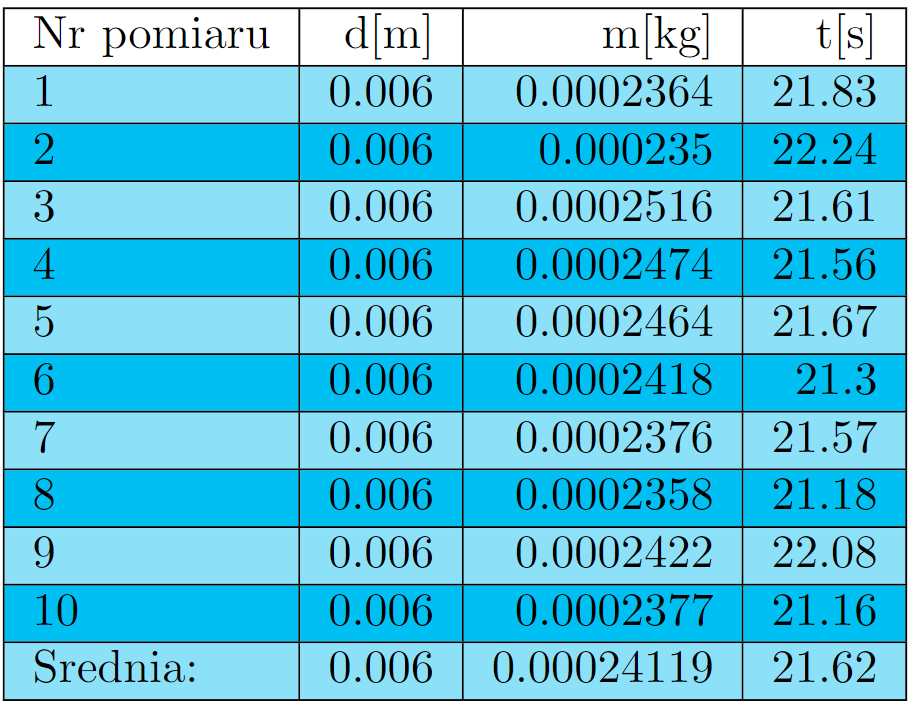
\includegraphics[width=0.9\linewidth, height=5cm]{t_niebieska_pom.png}
        \caption{Pomiary kulki Niebieskiej}
        \label{fig:subim2}
    \end{subfigure}
    \end{center}     
    % \caption{Caption for this figure with two images}
    % \label{fig:image2}
     \caption{Tabele dla kulki białej, czarnej i niebieskiej, kolejno}
\end{figure}
\noindent
Gęstość cieczcy została wyznaczona Areometrem:\\
$\rho_{c}=1330 \pm10 \ \left[\frac{kg}{m^{3}}\right]$\\
Gęstość kulki obliczamy z następującego wzoru:\\
$\rho_{k}=\frac{6m}{\pi d^{3}}$\\
Niepewność gęstości kulki:\\
$u_{c}(\rho_{k})=\sqrt{\left(\frac{6}{\pi d^{3}}\right)^{2}\cdot u^{2}(\bar{m}) + \left(\frac{12m}{\pi d^{4}}\right)\cdot u^{2}(d)}$\\
Wzór na niepewność lepkości:\\
$u(\eta)_{c}=u_{c}(y)=\sqrt{\sum^{k}_{j=1}\left(\frac{\partial f}{\partial x_{j}}\right)^{2}\cdot u^{2}(x_{j})}=  \\= \sqrt{\left(\frac{ 2\cdot d\cdot g\cdot \bar{t}\cdot (\rho_{k}-\rho_{c})  }{ 18h  }\right)^{2}\cdot u_{c}^{2}( d  )+
\left(\frac{ d^{2}\cdot g\cdot (\rho_{k}-\rho_{c})  }{ 18h  }\right)^{2}\cdot u_{c}^{2}( t  )+
\left(\frac{ d^{2}\cdot g\cdot \bar{t}  }{ 18h  }\right)^{2}\cdot u_{c}^{2}( \rho_{k}  )+
\left(\frac{ -d^{2}\cdot g\cdot \bar{t}  }{ 18h  }\right)^{2}\cdot u_{c}^{2}( \rho_{c}  )+
\left(\frac{ -d^{2}\cdot g\cdot (\rho_{k}-\rho_{c})  }{ 18h^{2}  }\right)^{2}\cdot u_{c}^{2}( h  )   }$\\
\noindent
Niepewność czasu:\\
$S_{\bar{t}}=\sqrt{\frac{1}{n(n-1)}\cdot\sum^{n}_{i=1}\left(t_{i}-\bar{t}\right)^{2}}$\\
Niepewność masy:\\
$S_{\bar{m}}=\sqrt{\frac{1}{n(n-1)}\cdot\sum^{n}_{i=1}\left(m_{i}-\bar{m}\right)^{2}}$\\
\newpage
\section{Przykładowe obliczenia}
Gęstość kulki:\\
$\rho_{k}=\frac{6\cdot 0.0004883}{\pi\cdot0.008^{3}}\approx1821.45\frac{kg}{m^{3}}$\\
Niepewność gęstości kulki:\\
$u_{c}(\rho_{k})=\sqrt{\left(\frac{6}{\pi\cdot 0.008^{3}}\right)^{2}\cdot 0.00000000004^{2}+\frac{12\cdot 0.0004883}{\pi\cdot 0.008^{4}}\cdot 0.00005^{2}}\approx35\frac{kg}{m^{3}}$\\
Niepewność czasu:\\
$S_{\bar{t}}=\sqrt{\frac{1}{10\cdot 9}\cdot 3,96444}\approx0.21s$\\
Lepkość:\\
$\eta=\frac{0.008^{2}\cdot 9.81\cdot 18.596\cdot (1821.45-1330)}{18\cdot 0.341}\approx0.94\frac{Ns}{m^{2}}$\\

%\begin{figure}
 %   \centering
  %  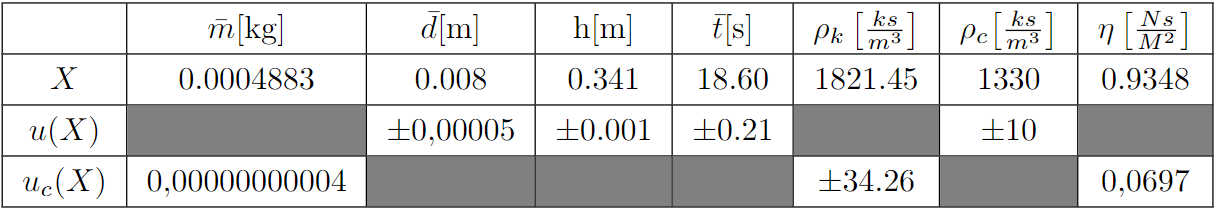
\includegraphics[scale=0.5]{t_b.png}
   % \caption{Wyliczone wartości, dla kulki Białej}
% \end{figure}
% \begin{figure}
    %\centering
    %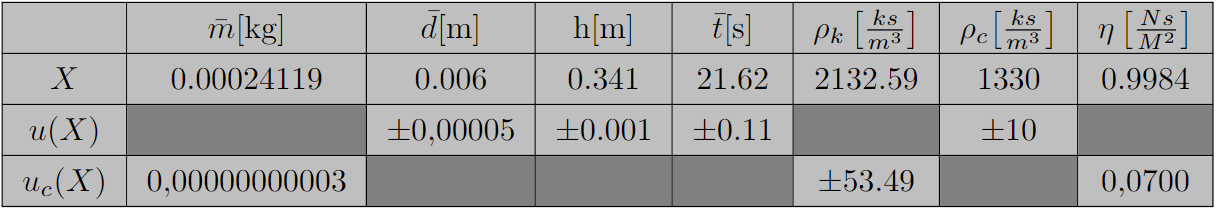
\includegraphics[scale=0.5]{t_c.png}
    %\caption{Wyliczone wartości, dla kulki Czarnej}
% \end{figure}
% \vspace{-10ex}
% \begin{figure}
    %\centering
    %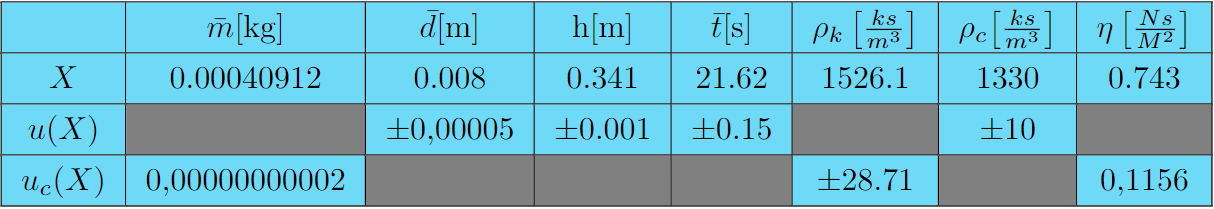
\includegraphics[scale=0.5]{t_n.png}
    %\caption{Wyliczone wartości, dla kulki Niebieskiej}
%\end{figure}
\begin{tabular}{|c|c|c|c|c|c|c|c|}
    \hline
    &$\bar{m}$[kg]&$\bar{d}$[m]&h[m]&$\bar{t}$[s]&$\rho_{k}\left[\frac{ks}{m^{3}}\right]$&$\rho_{c}$$\left[\frac{ks}{m^{3}}\right]$&$\eta\left[\frac{Ns}{M^{2}}\right]$\\
    \hline 
    $X$ &0.0004883&0.008&0.341&18.60&1821.45&1330&0.9348\\\hline
    % $\Delta X$&&&\\\hline
    $u(X)$&\cellcolor{gray}&$\pm$0.00005&$\pm$0.001&$\pm$0.21&\cellcolor{gray}&$\pm$10&\cellcolor{gray}    \\\hline
    $u_{c}(X)$&0.00000000004&\cellcolor{gray}&\cellcolor{gray}&\cellcolor{gray}&$\pm$34&\cellcolor{gray}&0.070\\\hline
    % 1&&&&&&&\hline
\end{tabular}
% 0.00005

\begin{tabular}{|c|c|c|c|c|c|c|c|}
    \hline
    \cellcolor{gray!50}&\cellcolor{gray!50}$\bar{m}$[kg]&\cellcolor{gray!50}$\bar{d}$[m]&\cellcolor{gray!50}h[m]&\cellcolor{gray!50}$\bar{t}$[s]&\cellcolor{gray!50}$\rho_{k}\left[\frac{ks}{m^{3}}\right]$&\cellcolor{gray!50}$\rho_{c}$$\left[\frac{ks}{m^{3}}\right]$&\cellcolor{gray!50}$\eta\left[\frac{Ns}{M^{2}}\right]$\\
    \hline 
    \cellcolor{gray!50}$X$ &\cellcolor{gray!50}0.00024119&\cellcolor{gray!50}0.006&\cellcolor{gray!50}0.341&\cellcolor{gray!50}21.62&\cellcolor{gray!50}2132.59&\cellcolor{gray!50}1330&\cellcolor{gray!50}0.9984\\\hline
    % $\Delta X$&&&\\\hline
    \cellcolor{gray!50}$u(X)$&\cellcolor{gray}&\cellcolor{gray!50}$\pm$0.00005&\cellcolor{gray!50}$\pm$0.001&\cellcolor{gray!50}$\pm$0.11&\cellcolor{gray}&\cellcolor{gray!50}$\pm$10&\cellcolor{gray}    \\\hline
    \cellcolor{gray!50}$u_{c}(X)$&\cellcolor{gray!50}0.00000000003&\cellcolor{gray}&\cellcolor{gray}&\cellcolor{gray}&\cellcolor{gray!50}$\pm$54&\cellcolor{gray}&\cellcolor{gray!50}0.070\\\hline
    % 1&&&&&&&\hline
\end{tabular}

\begin{tabular}{|c|c|c|c|c|c|c|c|}
    \hline
    \cellcolor{cyan!50}&\cellcolor{cyan!50}$\bar{m}$[kg]&\cellcolor{cyan!50}$\bar{d}$[m]&\cellcolor{cyan!50}h[m]&\cellcolor{cyan!50}$\bar{t}$[s]&\cellcolor{cyan!50}$\rho_{k}\left[\frac{ks}{m^{3}}\right]$&\cellcolor{cyan!50}$\rho_{c}$$\left[\frac{ks}{m^{3}}\right]$&\cellcolor{cyan!50}$\eta\left[\frac{Ns}{M^{2}}\right]$\\
    \hline 
    \cellcolor{cyan!50}$X$ &\cellcolor{cyan!50}0.00040912&\cellcolor{cyan!50}0.008&\cellcolor{cyan!50}0.341&\cellcolor{cyan!50}21.62&\cellcolor{cyan!50}1526.1&\cellcolor{cyan!50}1330&\cellcolor{cyan!50}0.743\\\hline
    % $\Delta X$&&&\\\hline
    \cellcolor{cyan!50}$u(X)$&\cellcolor{gray}&\cellcolor{cyan!50}$\pm$0.00005&\cellcolor{cyan!50}$\pm$0.001&\cellcolor{cyan!50}$\pm$0.15&\cellcolor{gray}&\cellcolor{cyan!50}$\pm$10&\cellcolor{gray}\\\hline
    \cellcolor{cyan!50}$u_{c}(X)$&\cellcolor{cyan!50}0.00000000002&\cellcolor{gray}&\cellcolor{gray}&\cellcolor{gray}&\cellcolor{cyan!50}$\pm$29&\cellcolor{gray}&\cellcolor{cyan!50}0.12\\\hline
    % 1&&&&&&&\hline
\end{tabular}
%Uzylem screenow zakomentowanych tablic bo za chuja nie wiem jak je ustawic
% % POMIARY KULKI BIALEJ
% \begin{minipage}{0.48\textwidth}
%     % \rowcolors{2}{gray!5}{lightgray!30}
%     \begin{table}
%         \caption{Wyniki pomiaru kulki Białej}
%         \begin{tabular}{|l|r|r|r|}
%             \hline
%             Nr & d[m] & m[kg] & t[s] \\ \hline
%             1 & 0.008 & 0.000486  & 18.61 \\ \hline
%             2 & 0.008 & 0.00048   & 18.48 \\ \hline
%             3 & 0.008 & 0.0004824 & 20.36 \\ \hline
%             4 & 0.008 & 0.0004844 & 18.18 \\ \hline
%             5 & 0.008 & 0.000498  & 18.14 \\ \hline
%             6 & 0.008 & 0.0004916 & 18.38 \\ \hline
%             7 & 0.008 & 0.0004924 & 18.9  \\ \hline
%             8 & 0.008 & 0.0004954 & 18.16 \\ \hline
%             9 & 0.008 & 0.0004812 & 18.25 \\ \hline
%             10& 0.008 & 0.0004916 & 18.5  \\ \hline
%             Srednia: & 0.008 & 0.0004883 & 18.596 \\ \hline
%         \end{tabular}%
%         \label{tab:Tabela Pomiarow Kulki Bialej}%
%     \end{table}%
% \end{minipage}
% % POMIARY KULKI BIALEJ


% % POMIARY KULKI CZARNEJ
% \begin{minipage}{0.48\textwidth}
%     % \rowcolors{2}{gray!70}{lightgray!80}
%     \begin{table}
%         \caption{Wyniki pomiaru kulki Czarnej}
%         \begin{tabular}{|l|r|r|r|}
%             \hline
%             Nr& d[m] & m[kg] & t[s] \\ \hline
%             1 & 0.006 & 0.0002364 & 21.83 \\ \hline
%             2 & 0.006 & 0.000235  & 22.24 \\ \hline
%             3 & 0.006 & 0.0002516 & 21.61 \\ \hline
%             4 & 0.006 & 0.0002474 & 21.56 \\ \hline
%             5 & 0.006 & 0.0002464 & 21.67 \\ \hline
%             6 & 0.006 & 0.0002418 & 21.3  \\ \hline
%             7 & 0.006 & 0.0002376 & 21.57 \\ \hline
%             8 & 0.006 & 0.0002358 & 21.18 \\ \hline
%             9 & 0.006 & 0.0002422 & 22.08 \\ \hline
%             10& 0.006 & 0.0002377 & 21.16 \\ \hline
%             Srednia: & 0.006 & 0.00024119 & 21.62 \\ \hline
%         \end{tabular}%
%         \label{tab:Tabela Pomiarow Kulki Czarnej}%
%     \end{table}%
% \end{minipage}
% % POMIARY KULKI CZARNEJ

% % \vspace{-50ex}
% % POMIARY KULKI NIEBIESKIEJ
% % \begin{minipage}[0.33\textwidth]
% %     \rowcolors{2}{cyan!90}{cyan!40}
% %     \begin{table}[h]    
% %         \caption{Wyniki pomiaru kulki Niebieskiej}
% %         \begin{tabular}{|l|r|r|r|}
% %             \hline
% %             Nr pomiaru & d[m] & m[kg] & t[s] \\ \hline
% %             1 & 0.006 & 0.0002364 & 21.83 \\ \hline
% %             2 & 0.006 & 0.000235  & 22.24 \\ \hline
% %             3 & 0.006 & 0.0002516 & 21.61 \\ \hline
% %             4 & 0.006 & 0.0002474 & 21.56 \\ \hline
% %             5 & 0.006 & 0.0002464 & 21.67 \\ \hline
% %             6 & 0.006 & 0.0002418 & 21.3  \\ \hline
% %             7 & 0.006 & 0.0002376 & 21.57 \\ \hline
% %             8 & 0.006 & 0.0002358 & 21.18 \\ \hline
% %             9 & 0.006 & 0.0002422 & 22.08 \\ \hline
% %             10& 0.006 & 0.0002377 & 21.16 \\ \hline
% %             Srednia: & 0.006 & 0.00024119 & 21.62 \\ \hline
% %         \end{tabular}%
% %         \label{tab:Tabela Pomiarow Kulki Niebieskiej}%
% %     \end{table}%
% % \end{minipage}
% % POMIARY KULKI NIEBIESKIEJ

% \newpage

% OTRZYMANE POMIARY I ICH OPRACOWANIE
%------------------------------------------------------------------

\section{Wnioski}
\begin{itemize}
    \item Na podstawie pomiarów lepkość cieczy wyszła w przybliżeniu lepkości gliceryny
    \item Wyniki nie są dokładne, ponieważ w roztworze mogła znajdować się woda
    \item Czas reakcji człowieka oraz że kulki nie są idealnymi kulami są powodami dużych różnic w czasach opadania kulki
    \item Wyniki lepkości wyznaczonej ze wzorów różnią się z powodu dużych niepeności pomiarowych masy i obwodu kulek
\end{itemize}
\end{document}
